%% For double-blind review submission, w/o CCS and ACM Reference (max submission space)
\documentclass[sigplan,10pt]{acmart}

\usepackage{graphicx}
%\usepackage[labelfont=bf]{caption}
%\usepackage[superscript,nomove]{cite}
%\usepackage{color}
%\usepackage{url}
%\usepackage{footnote}
\usepackage{comment}
\usepackage{todonotes}
\usepackage{booktabs}
\usepackage{siunitx}

\settopmatter{printfolios=true,printccs=false,printacmref=false}

%% For double-blind review submission, w/ CCS and ACM Reference
%\documentclass[sigplan,review,anonymous]{acmart}\settopmatter{printfolios=true}

%% For single-blind review submission, w/o CCS and ACM Reference (max submission space)
%\documentclass[sigplan,review]{acmart}\settopmatter{printfolios=true,printccs=false,printacmref=false}

%% For single-blind review submission, w/ CCS and ACM Reference
%\documentclass[sigplan,review]{acmart}\settopmatter{printfolios=true}

%% For final camera-ready submission, w/ required CCS and ACM Reference
%\documentclass[sigplan]{acmart}\settopmatter{}


%% Conference information
%% Supplied to authors by publisher for camera-ready submission;
%% use defaults for review submission.
\acmConference[SIGTBD]{}
\acmYear{CSAIL, MIT, USA, 2019}
\acmISBN{} % \acmISBN{978-x-xxxx-xxxx-x/YY/MM}
\acmDOI{} % \acmDOI{10.1145/nnnnnnn.nnnnnnn}
\startPage{1}

%% Copyright information
%% Supplied to authors (based on authors' rights management selection;
%% see authors.acm.org) by publisher for camera-ready submission;
%% use 'none' for review submission.
\setcopyright{none}
%\setcopyright{acmcopyright}
%\setcopyright{acmlicensed}
%\setcopyright{rightsretained}
%\copyrightyear{2018}           %% If different from \acmYear

%% Bibliography style
\bibliographystyle{ACM-Reference-Format}
%% Citation style
%\citestyle{acmauthoryear}  %% For author/year citations
%\citestyle{acmnumeric}     %% For numeric citations
%\setcitestyle{nosort}      %% With 'acmnumeric', to disable automatic
                            %% sorting of references within a single citation;
                            %% e.g., \cite{Smith99,Carpenter05,Baker12}
                            %% rendered as [14,5,2] rather than [2,5,14].
%\setcitesyle{nocompress}   %% With 'acmnumeric', to disable automatic
                            %% compression of sequential references within a
                            %% single citation;
                            %% e.g., \cite{Baker12,Baker14,Baker16}
                            %% rendered as [2,3,4] rather than [2-4].


%% Some recommended packages.
\usepackage{booktabs}   %% For formal tables:
                        %% http://ctan.org/pkg/booktabs
\usepackage{subcaption} %% For complex figures with subfigures/subcaptions
                        %% http://ctan.org/pkg/subcaption


\begin{document}

%% Title information
\title[Good Dog Human Baselines]{Human Baseline for Zero-Shot Transfer Learning of Good Dogs}         %% [Short Title] is optional;
                                        %% when present, will be used in
                                        %% header instead of Full Title.
%\titlenote{}             %% \titlenote is optional;
                                        %% can be repeated if necessary;
                                        %% contents suppressed with 'anonymous'
%\subtitle{or, why we're so good with dogs}                     %% \subtitle is optional
%\subtitlenote{with subtitle note}       %% \subtitlenote is optional;
                                        %% can be repeated if necessary;
                                        %% contents suppressed with 'anonymous'


%% Author information
%% Contents and number of authors suppressed with 'anonymous'.
%% Each author should be introduced by \author, followed by
%% \authornote (optional), \orcid (optional), \affiliation, and
%% \email.
%% An author may have multiple affiliations and/or emails; repeat the
%% appropriate command.
%% Many elements are not rendered, but should be provided for metadata
%% extraction tools.

%% Author with single affiliation.
\author{William Boag, Shashank Srikant}
%\authornote{with author1 note}          %% \authornote is optional;
                                        %% can be repeated if necessary
%\orcid{nnnn-nnnn-nnnn-nnnn}             %% \orcid is optional
\affiliation{
  %\position{PhD Student}
  %\department{Department1}              %% \department is recommended
  \institution{MIT CSAIL}            %% \institution is required
  %\streetaddress{Street1 Address1}
  \city{Cambridge}
  \state{MA}
  %\postcode{Post-Code1}
  \country{USA}                    %% \country is recommended
}
\email{{wboag,shash}@mit.edu}          %% \email is recommended



%% Abstract
%% Note: \begin{abstract}...\end{abstract} environment must come
%% before \maketitle command
\begin{abstract}
It is estimated that there are 900 million dogs in the world. That is a lot of dogs, and we assure you that each one is a good dog \cite{dog-rates}. Unfortunately, we don't have enough time to meet each dog de novo, and have inevitably needed to rely on word-of-mouth to learn about which dogs to meet and when. In this work, we demonstrate human-level performance for zero-shot dog recognition from features described by other humans. Human performance is robust (>85\% accuracy), even when presented with challenging comparisons. This accuracy is in the same ballpark as Karpathy et al.'s work on a human baseline for ImageNet \cite{karpathy}. We believe that this work will help future researchers develop AI-based tools for super-human performance on word-of-mouth-based human-dog introductions. From a neuroscience perspective, this work also establishes the presence of a seeming information barrier between the visual cortex and the language system of the human brain.
\end{abstract}





%% Keywords
%% comma separated list
\keywords{Good Dogs, Zero-Shot Transfer Learning, Human Performance, Visual Cortex, Language Processing}  %% \keywords are mandatory in final camera-ready submission


%% \maketitle
%% Note: \maketitle command must come after title commands, author
%% commands, abstract environment, Computing Classification System
%% environment and commands, and keywords command.
\maketitle



\section{Introduction}
There are so many dogs. It is a very exciting time to be alive, for sure. But with great opportunities come great opportunity costs: \textbf{the average citizen simply does not have enough time to meet every dog cold.} Typically, we get to know dogs through a third-party, usually starting with a verbal description. Many dogs are never photographed, which makes sense because very few dogs have sufficient Instagram followings. Dogs like Doug the Pug \cite{doug-the-pug} are the exception rather than the rule. Most dogs are more like hidden gems, rather than national crown jewels. As such, it is critical that we are able to rely on verbal descriptions of dogs in order to learn which dog we will be meeting.

\begin{figure}[h!]
    \center{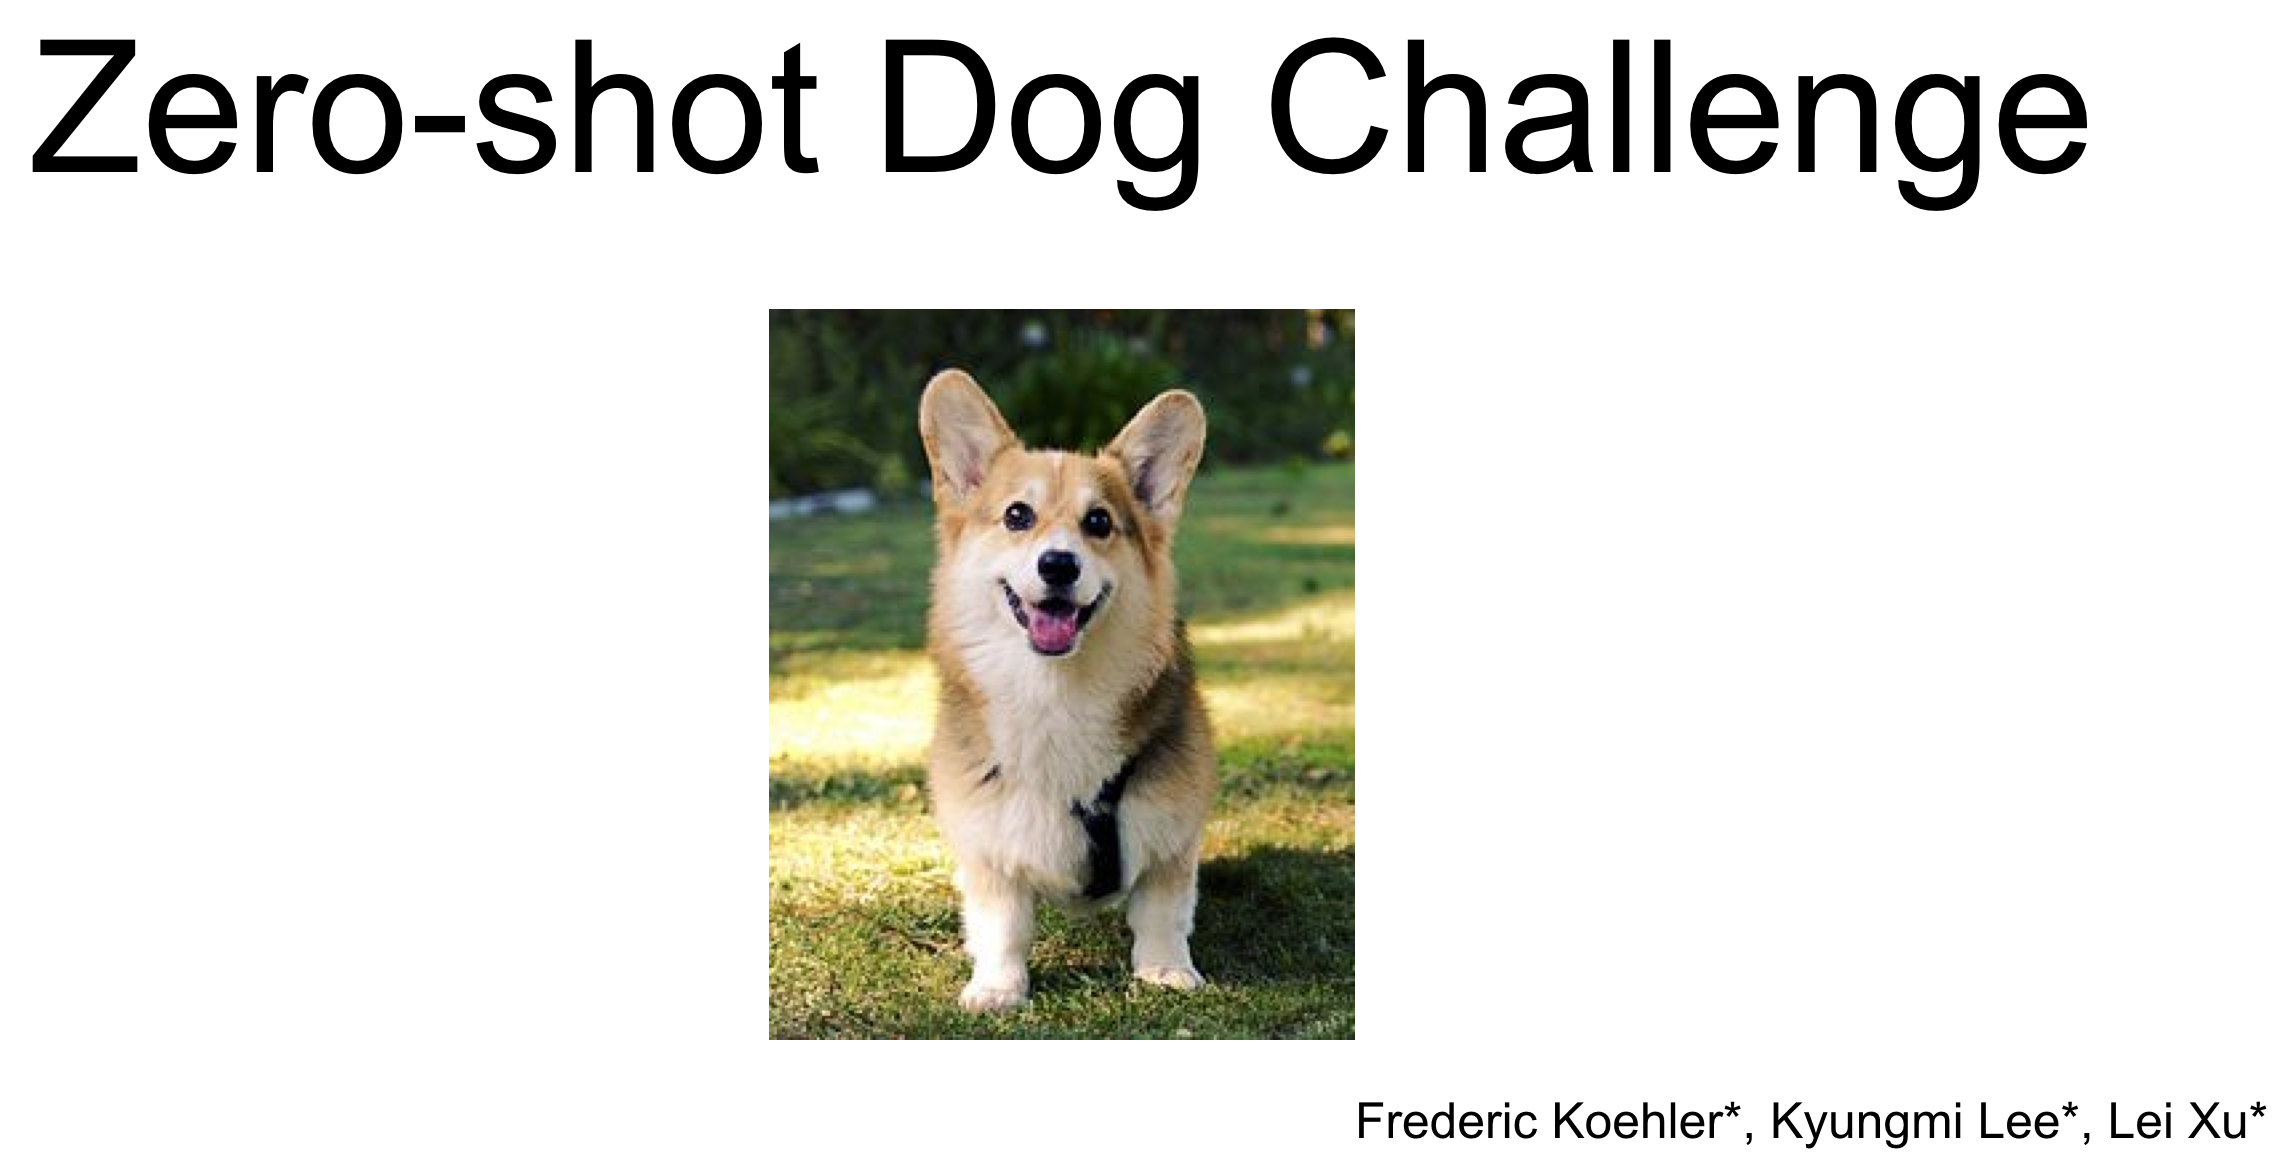
\includegraphics[width=0.46\textwidth]{images/cover.png}}
    \caption{Cover for the Zero-shot Dog Challenge slide deck}
    \label{fig:cover}
\end{figure}

Everyone knows that technology-driven solutions will facilitate human-dog interactions, but it has not been rigorously studied how well humans perform on this task (and therefore what the value-add would be for AI-based technologies). In this work, we provide the much-needed empirical analysis of how well humans are able to identify dogs based on just verbal descriptions. We expect that with this groundwork laid, there will be an uptick in both research grants and startups for Computational Dog-related Studies. We speculate that this will likely be a hot area of research in the future.

Skeptics argue that these are problems of the past and that technology will enable picture-based social media networks for meeting dogs. In fact, there have been attempts of this in recent years such as \textit{Tinder for Dogs} \cite{tindog} and \textit{Meet My Dog App} \cite{meetmydog}. However, these technocrats overlook basic, fundamental flaws with this approach. For starters, some dogs are shy and don't want their photos online. In addition, no courts have ruled whether the Fourth Amendment (United States) or GDPR (European Union) applies to dogs. The United States legal system has recognized that some animals do have standing to bring suits in federal courts \cite{monkey-standing}, so the matter of whether dogs have a legal right to privacy is currently unresolved. Nevertheless, such tools will not solve all of our problems.

\begin{figure*}[!htb]
\minipage{0.68\textwidth}
    \center{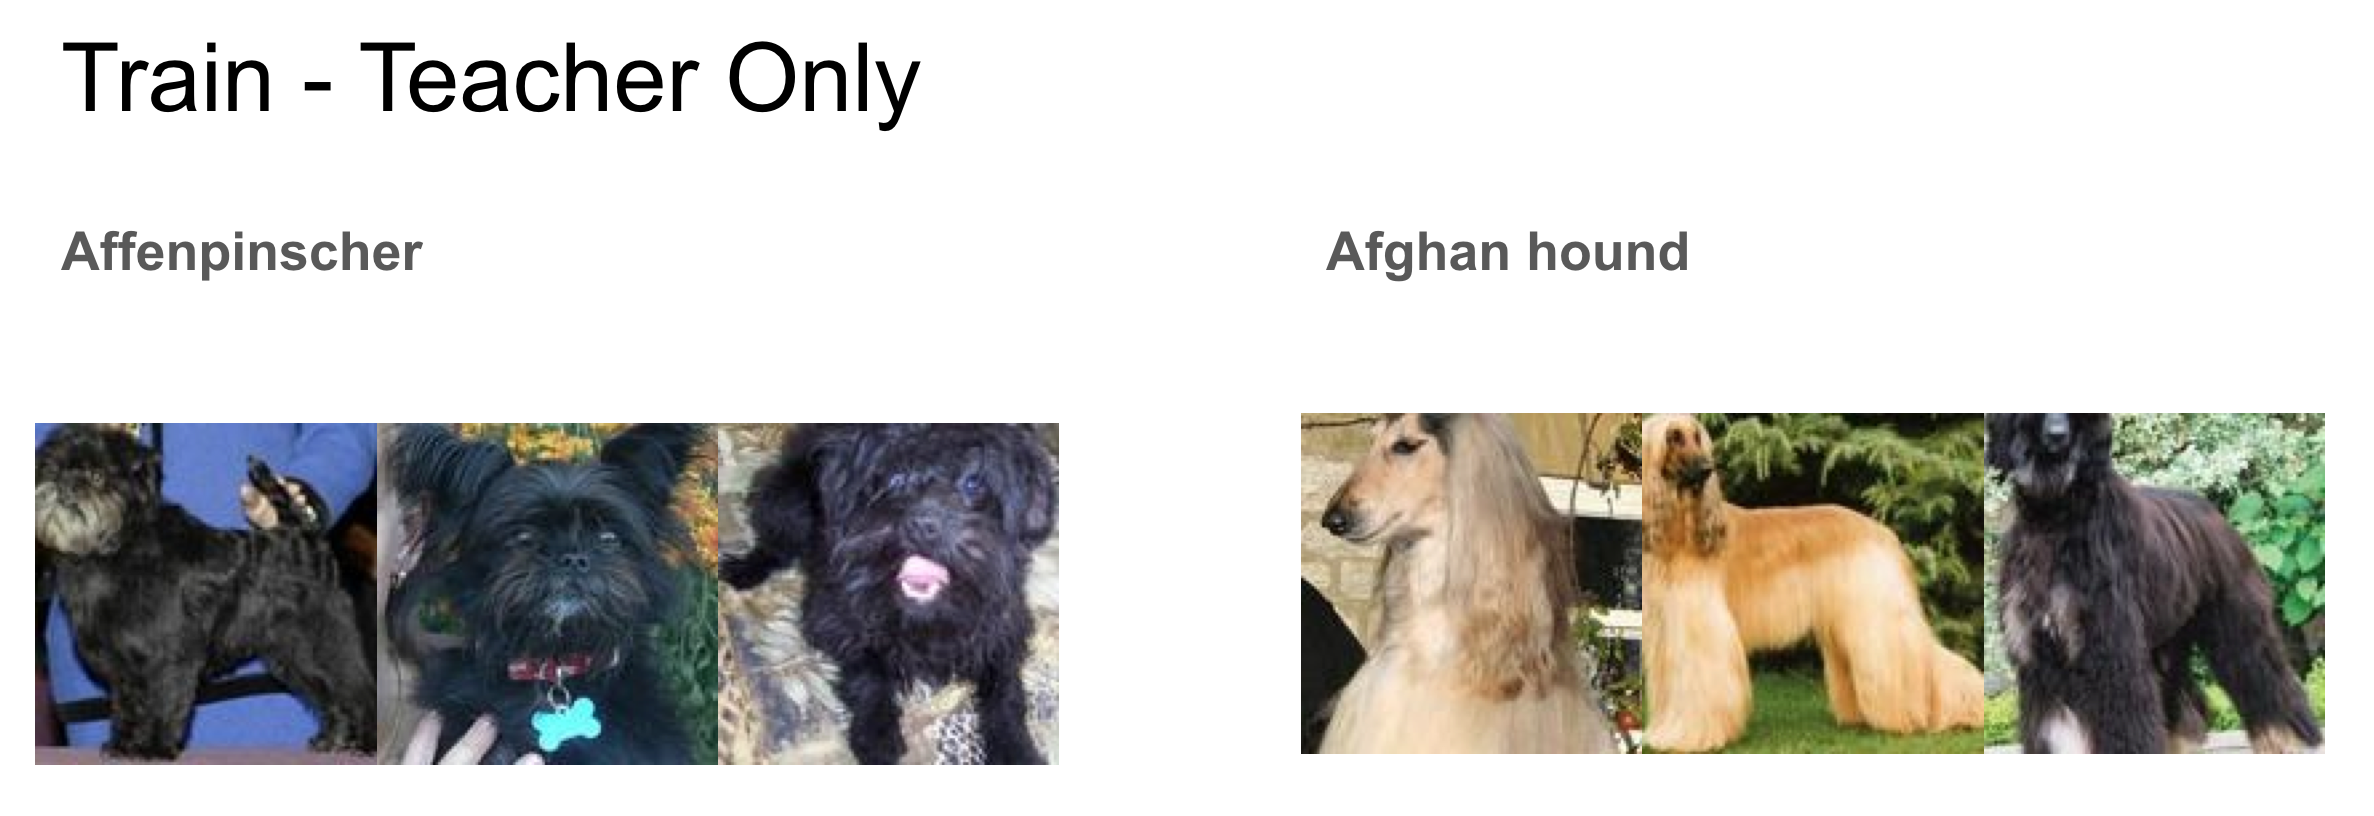
\includegraphics[width=\textwidth]{images/example-train.png}}
    \caption{Example training slide shown to a teacher.}
    \label{fig:example-train}
\endminipage\hfill
\minipage{0.32\textwidth}%
    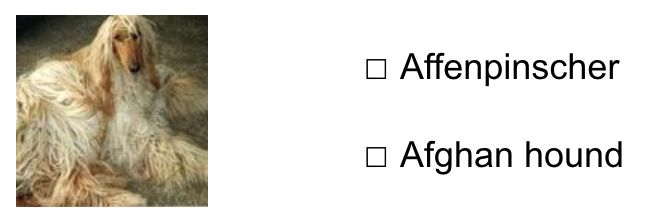
\includegraphics[width=1.2\textwidth]{images/example-test.png}
    \caption{Example prediction slide shown to a team.}
    \label{fig:example-test}
\endminipage
\caption{\textbf{Task details.} Two breeds of dogs, each with 3-5 images, were displayed to the \textit{teacher} from each team. The rest of the team would not have access to these images while the \textit{teacher} viewed this set of images. The \textit{teacher} would then have to explain the breeds to the team. The teams would then be shown a test image and would be asked to guess the breed.}
\end{figure*}
Our contributions in this work are as follows
\begin{itemize}
    \item We show that humans are pretty good at identifying dog breeds based on verbal comparative descriptions. These descriptions are produced by observing just 2-3 images of the dogs in question (and hence, zero-shot).
    \item By quantifying the performance of humans on a zero-shot transfer learning task, we establish a bound on what can possibly be performed by an AI technology designed for such tasks.
    \item We hypothesize that there exists a barrier between the information processed by the visual cortex, and the processed information being available to the language system of the human brain.
\end{itemize}


\section{Previous Work}
SIG TBD is home to seminal work in the field of Machine Learning for Dogs: Boag (2018) empirically proved that every dog in Cambridge, MA is a good dog \cite{good-dogs}, though it is still an open problem whether this has a theoretical basis to it.

In 2018, Kaggle unveiled a competition for Dog Breed Identification Challenge \cite{kaggle-breed-classification}. Similarly, Machine Learning techniques have been deployed for app-based breed classification \cite{ml-breed-classification}. Of course for all of these works, there is always an extensive training set to learn from hundreds of examples per class. This requires a lot of effort.

Dog-based Machine Learning has also arguably been studied in fields like Interpretable AI. Specifically, there are some works which used multiple pictures of dogs in their Computer Vision papers \cite{interpretable-dogs}. There may be other such papers as well.

More recently, attempts have been made to learn machine learning models through comparison \cite{cmu}. This is closest in spirit to the human neural activity that the zero-shot transfer learning task in our work engages.


\section{Methods}

\subsection{The Task}

In February 2019, the authors participated in a competition among humans for zero-shot dog breed classification. The rules were as follows:

\begin{enumerate}
\item 5 rounds of game per team (each team comprised 6 people)
\item In each round, one person from a team will be a ``teacher''. The teacher is shown two dog breeds. For each breed, 2-5 images are shown. S/he is given 30 seconds to look at the two sets of images, and 30 seconds to describe the two breeds based on their observation.
\item The organizers then choose on unseen image of any of the two breeds and show it to the team members. Based on the descriptions they heard, the team members are now required to guess which of the two breeds the dog belongs to. They have a 50\% probability of getting it right. They are then given 20 seconds to think/deliberate/discuss. Importantly, they have no access to the `training set' which the teacher had access to.
\item All images are from Stanford Dogs Dataset \cite{dognet}
\end{enumerate}


An example of this procedure can be seen in Figures \ref{fig:example-train} (teacher training) and \ref{fig:example-test} (prediction slide). In this case, the teacher (while looking at Figure \ref{fig:example-train}) might describe the difference between the dogs as ``Affenpinschers are always black, whereas Afghan Hounds can sometimes be black and sometimes be brown'' or perhaps ``The Afghan Hound is a lot larger than the Affenpinscher.'' After the teacher describes the differences for 30 seconds, the team then sees Figure \ref{fig:example-test} and must deliberate to decide whether the dog is an Affenpinscher or Afghan Hound.


\subsection{Teams}

There were three teams that participated in this competition. Although all teams followed the same framework (i.e. take notes while teacher describes dogs and then reference those notes during prediction time), they employed different strategies for their predictions. The first team had seemingly a dog expert and usually listened to that teammate's recommendation for predictions. The second team adopted an ensemble approach in which everyone independently made their predictions before discussing (in an effort to combat group think). The third team did all of their deliberation in Chinese because that was their native language, and was therefore easier for them to communicate.


\begin{figure*}[!h]
\minipage{0.68\textwidth}
    \center{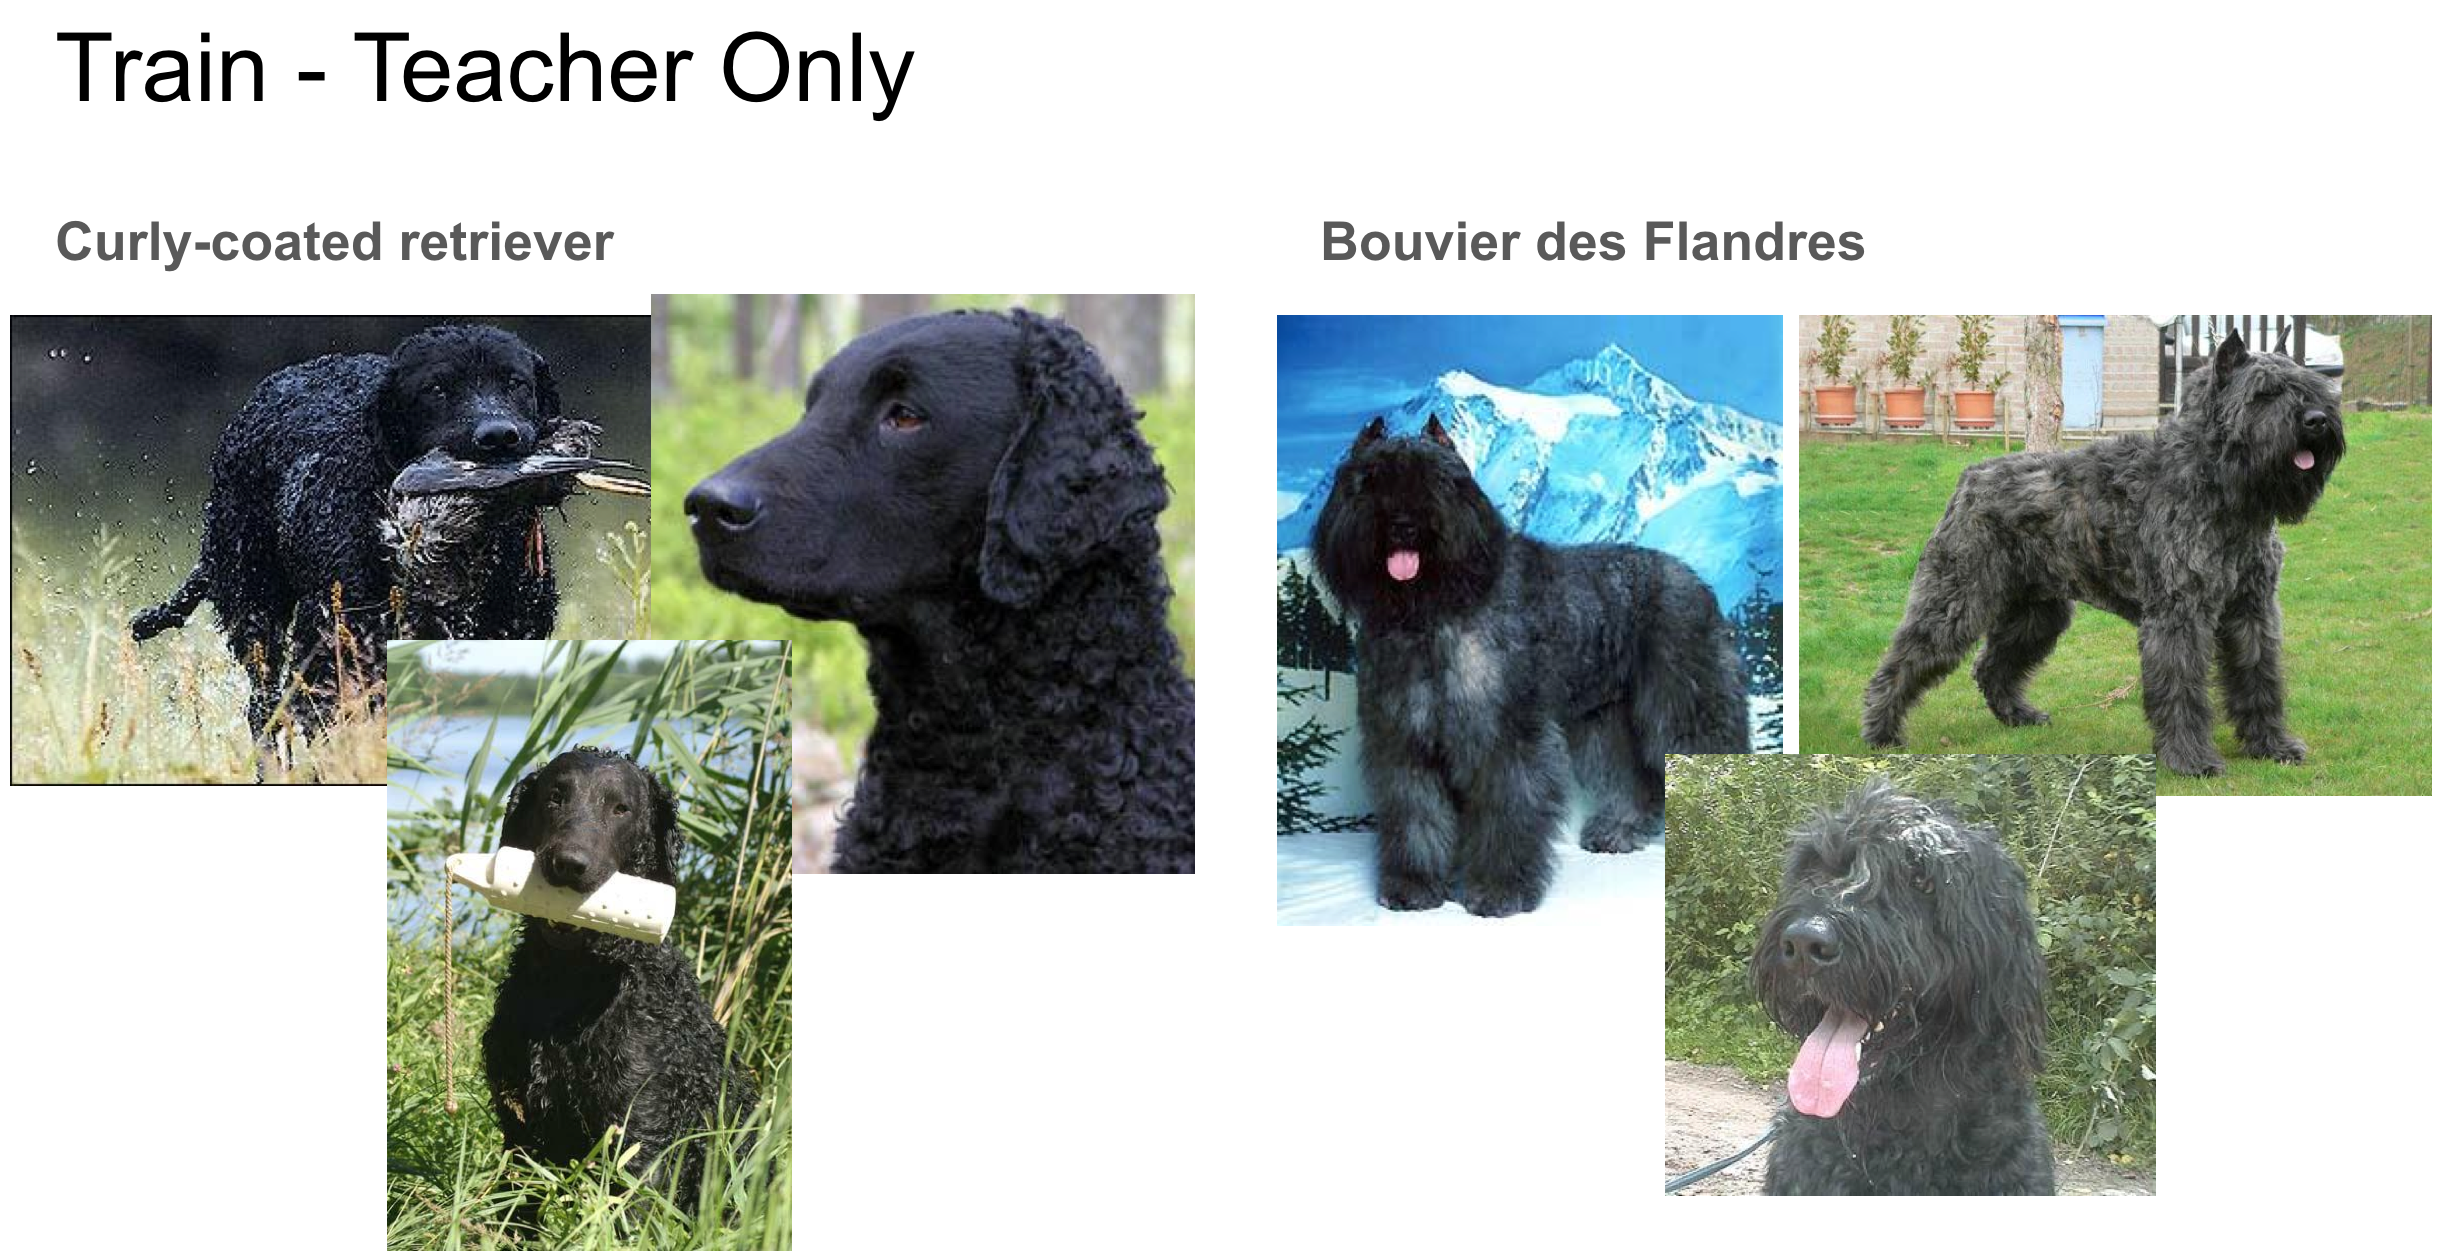
\includegraphics[width=\textwidth]{images/ex1-train.png}}
    \caption{Example training slide for team 2.}
    \label{fig:team2-train}
\endminipage\hfill
\minipage{0.32\textwidth}%
    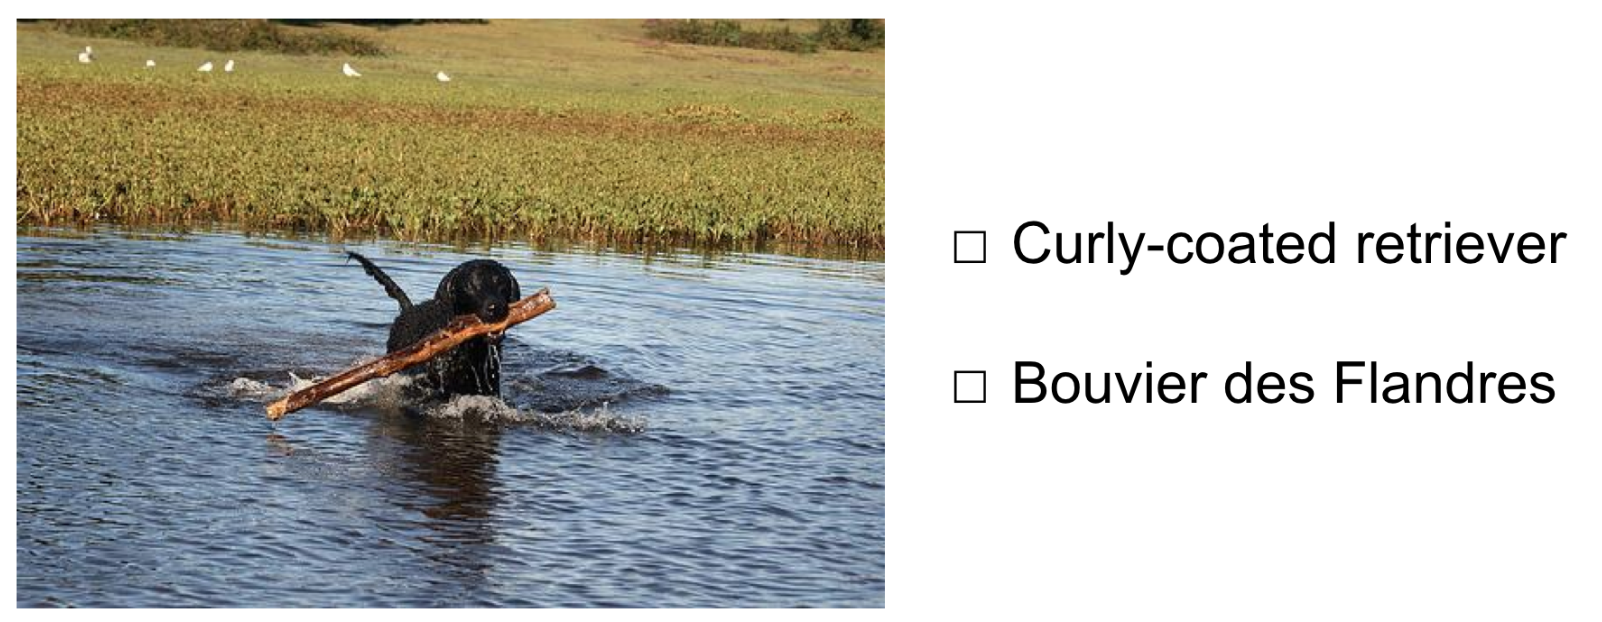
\includegraphics[width=1.2\textwidth]{images/ex1-test.png}
    \caption{Prediction slide for the task from Figure \ref{fig:team2-train}}
    \label{fig:team2-test}
\endminipage
\caption{\textbf{Perils of a correlation-based predictor being illustrated by humans.} On showing images of curly-coated retrievers and Bouvier des Flanders, one of the teams' teachers described an incorrect \textit{feature} to their team - of retrievers generally holding onto an object in their mouths. Coincidentally, the prediction image consisted of a retriever conveniently holding an object in its mouth, leading their team to guess that the good dog was a retriever. This demonstrates how learning a correlating feature which is not causal can have dire consequences in modern AI systems.}
\end{figure*}


\section{Results}

Humans performed surprisingly well. All three teams got $\frac{7}{8} (=87.5\%)$ predictions right. This is in the same range as human baseline results reported by Karpathy et al. for ImageNet \cite{karpathy}. Notes from all three teams are shown in Figures \ref{fig:notes1}, \ref{fig:notes2}, and \ref{fig:notes3}. 

Analyzing the notes revealed interesting information. One note from team 1 (not shown here) suggested that some teammates were more visually inclined than others, as they chose to draw the descriptions provided by their teacher rather than writing them out. This seems to have played no difference in the final accuracy though.

We can see in Figure \ref{fig:notes2} that the ensemble-based approach gives 6 times as many labels for the human baseline. 
Further, we can see that most team predictions were unanimous (6-0) or near unanimous (5-1), showing the predictions were not independent (and therefore all based in the same direction), thus defeating the noise cancelling benefits of ensembling.

\section{Discussion}
\subsection{Dog descriptions}
There were some very good human descriptions of the dogs, including:
\begin{enumerate}
    \item ``It's super cute and fluffy when it is small.''
    \item ``The Corgi... looks like a dwarf. Like a dog meets a dwarf... in it's legs.''
    \item ``They're very different. But each beautiful creatures in their own right.''
\end{enumerate}


\subsection{Perils of correlation-based prediction systems}
Occasionally, humans were arguably right for the wrong reasons. The teacher who was describing the classes in Figure \ref{fig:team2-train} confidently stated that Curly-coated Retrievers ``almost always are holding something in their mouths.'' Lo and behold, the prediction image (shown in Figure \ref{fig:team2-test}) showed a Curly-coated retriever holding something in its mouth. This suggests a potential downside to such feature-based, correlation-driven prediction systems. It is, of course, possible that this property is a true fact about the world. More research is required to establish its certainty.


\subsection{Neuroscience of zero-shot transfer learning}
This task opens up the possiblity of the existence of an information barrier between what is processed by the visual cortex, and how much of it can be retrieved by the language system in the human brain. In this task, the teacher observes images of the two breeds, processes it, and is required to then switch to using her/his language system to describe what they just perceived. Neuroscientifically, this requires the brain to distill a representation of the two breeds from the visual cortex, which is then supposedly accessed by the language system. In our tasks, we observe that each task from each team had less than a 100\% accuracy, which suggests that the language system cannot potentially access all the information processed by the visual cortex. In a sense, there possibly exists an information barrier between the representation that is encoded by the visual cortex, and the information decoded from it by the language system. Such a lossy decoding is indicative of the brain using a low dimension feature space (as compared to the feature space enabled by retinal ganglion cells) to store such representations. As a caveat, the statistical validity of these results are limited ($n=6$ subjects). This is a possible research question which can be tested through behavioral studies in the future.

\section{Conclusion}

All dogs are, and will remain good. Additionally, people are pretty good at identifying dogs without having seen them before. We speculate that assistive technology could help humans perform even better, thus allowing people to achieve super-human performance at identifying dogs. This could enable future citizens of the world to meet more dogs than ever imagined.



%% Acknowledgments
\begin{acks}
We thank the \textit{ML Across MIT} organizing committee (especially Kyungmi Lee, Lei Xu, and Frederic Koehler) for putting this fun challenge together.

\end{acks}


%% Bibliography
\bibliography{refs}

%% Appendix
\appendix
\section{Appendix}

\begin{figure*}
    \center{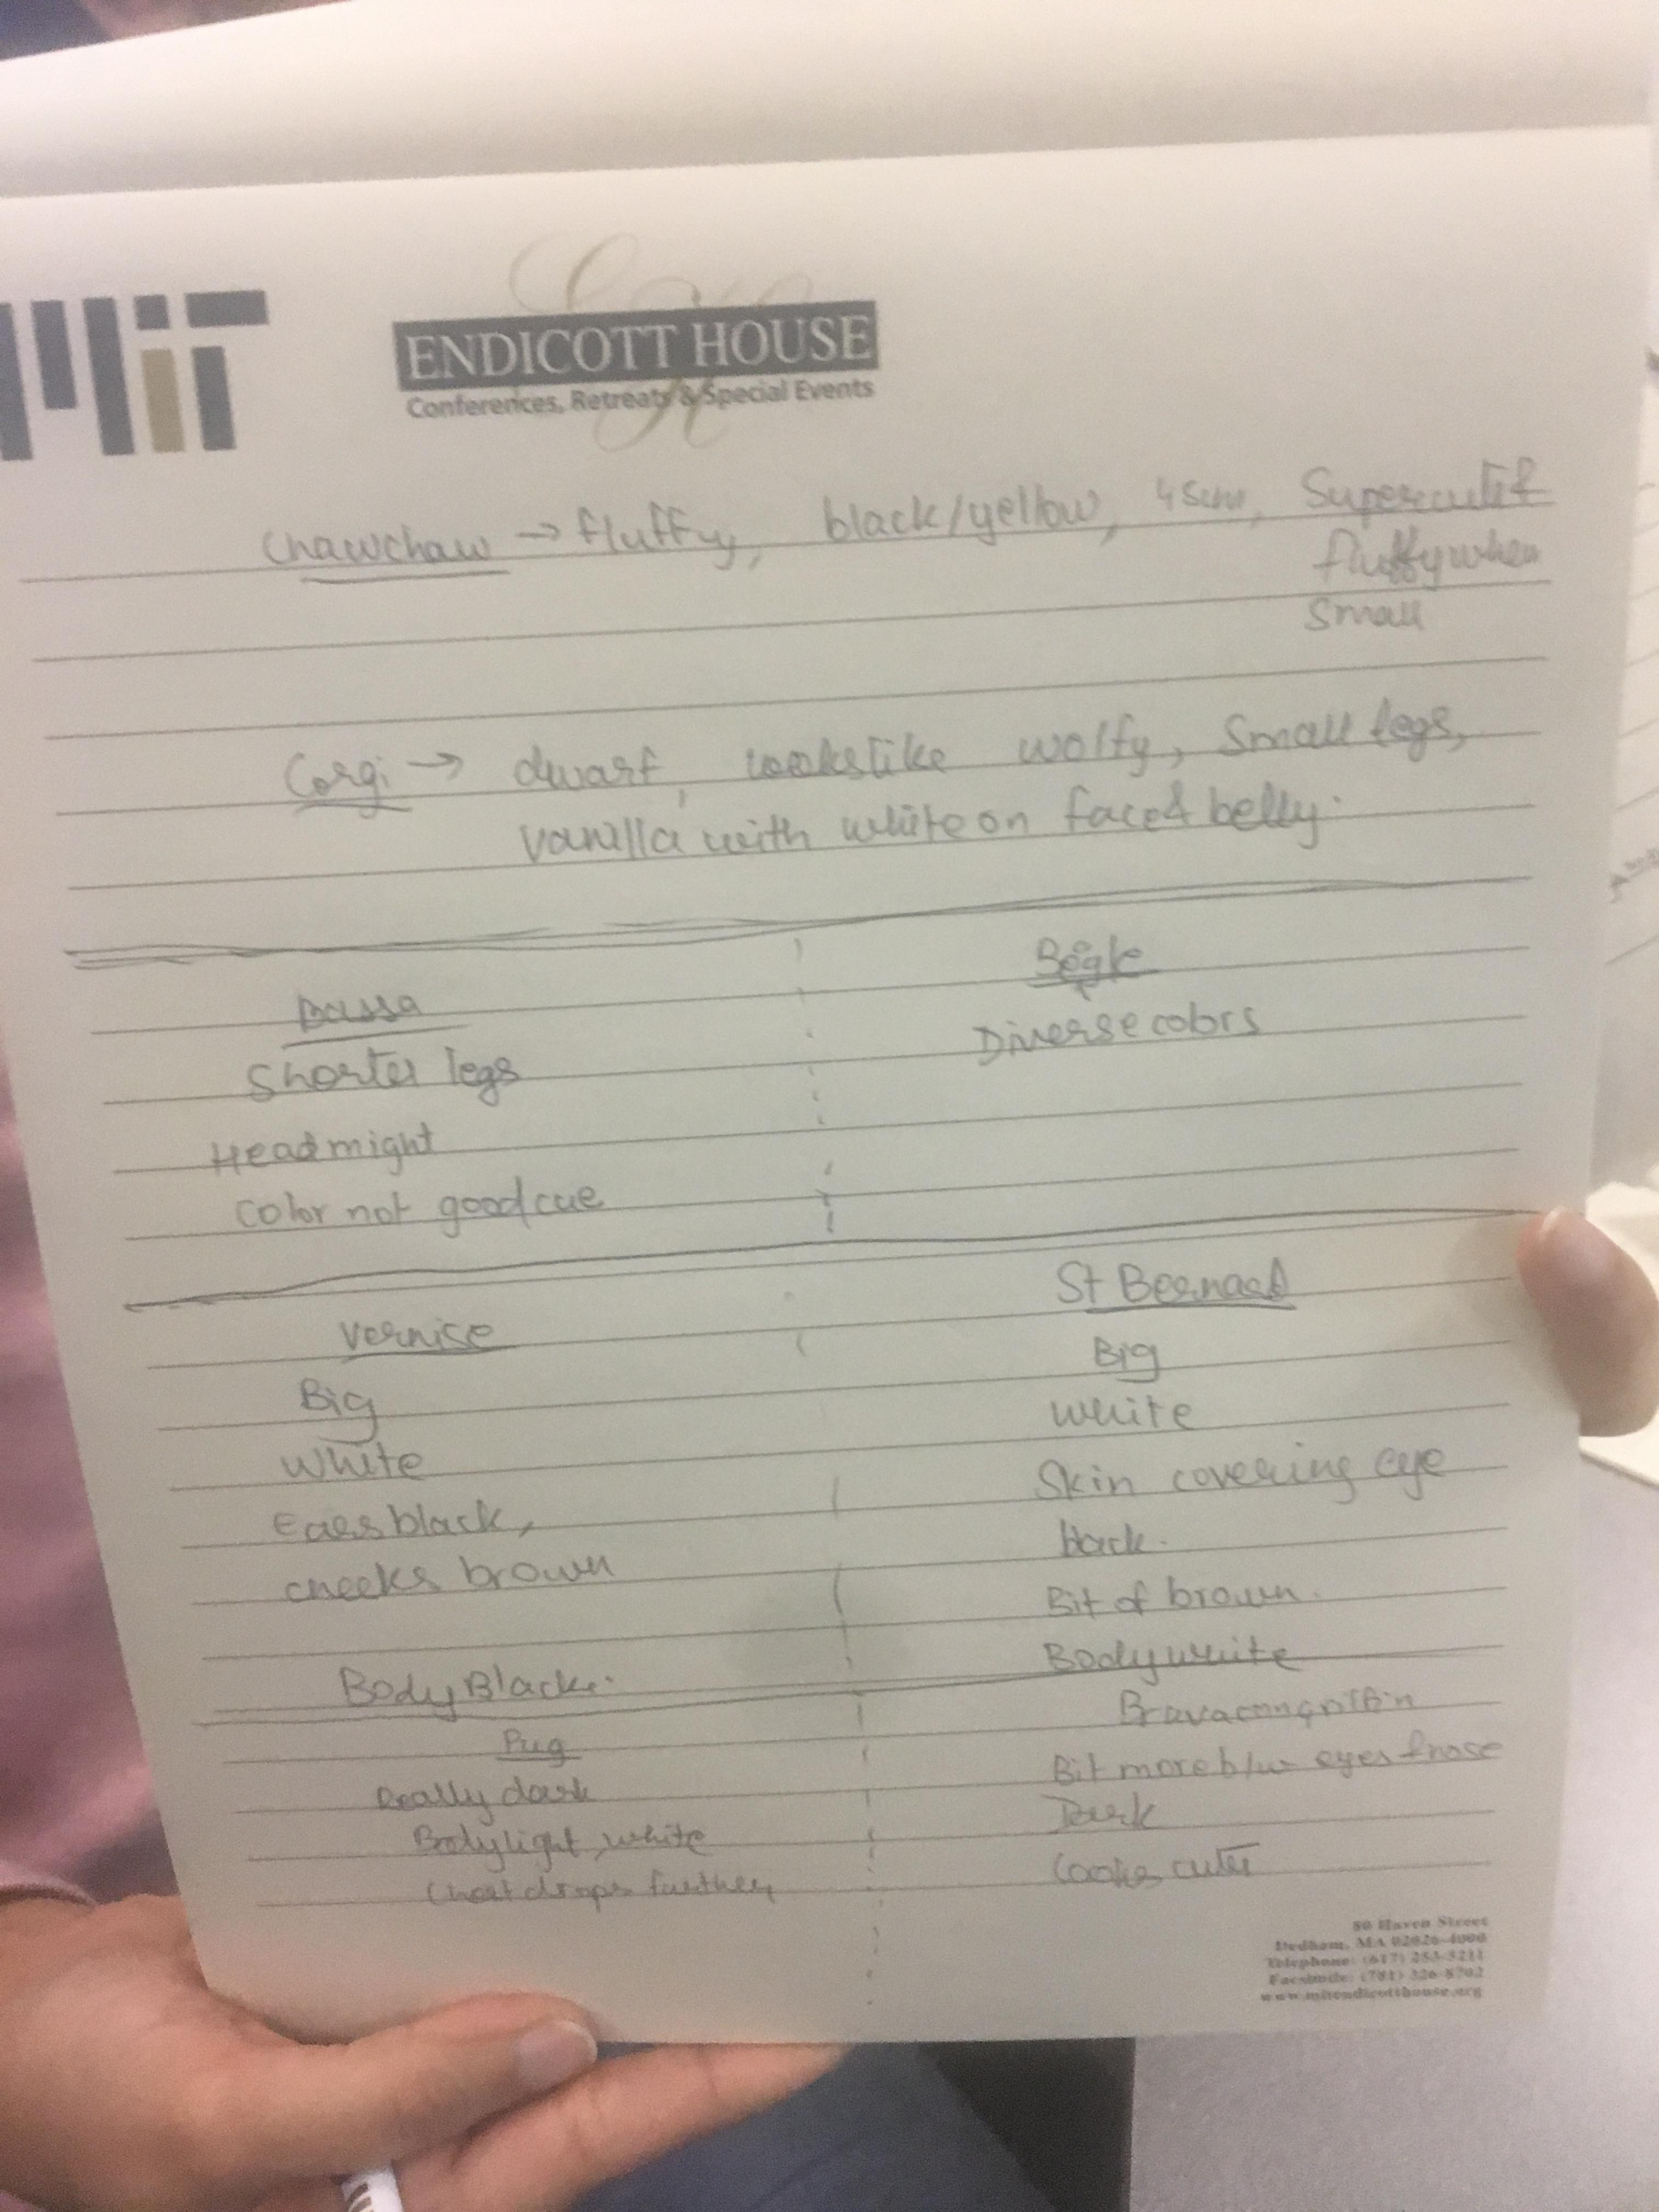
\includegraphics[width=0.89\textwidth]{images/notes-1.jpg}}
    \caption{Notes taken by a member of team 1.}
    \label{fig:notes1}
\end{figure*}

\begin{figure*}
    \center{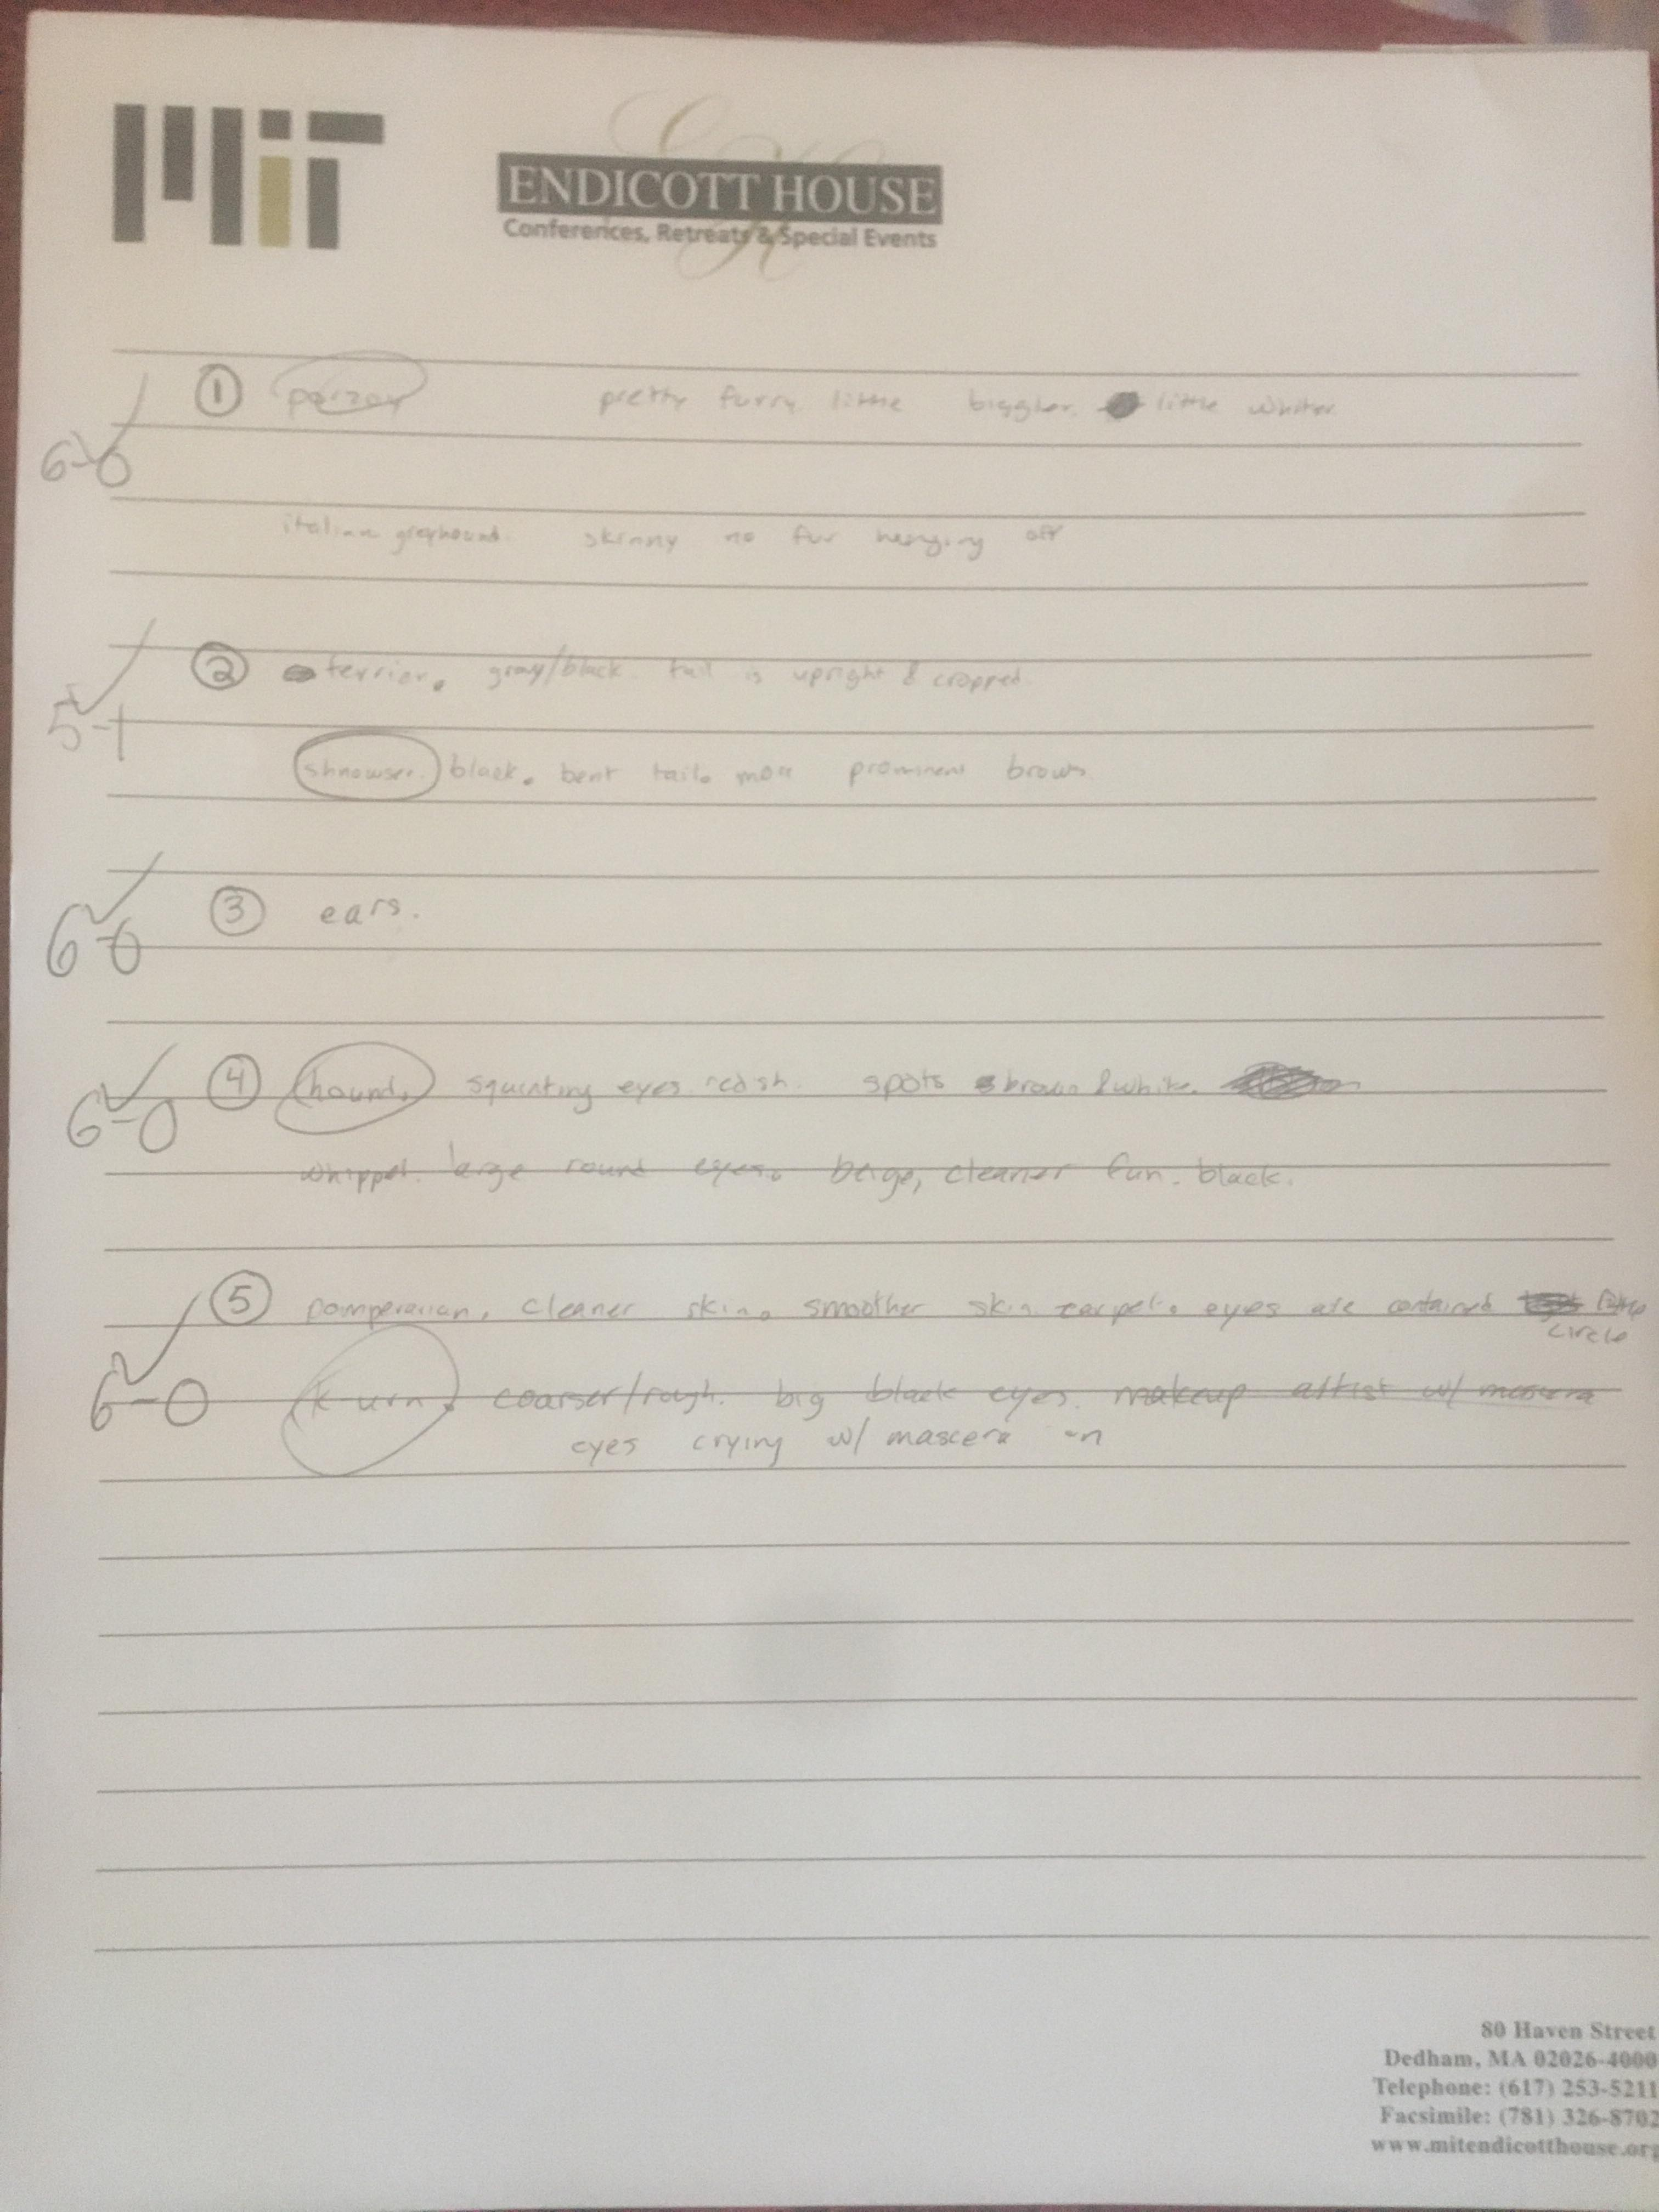
\includegraphics[width=0.89\textwidth]{images/notes-2.jpg}}
    \caption{Notes taken by a member of team 2.}
    \label{fig:notes2}
\end{figure*}

\begin{figure*}
    \center{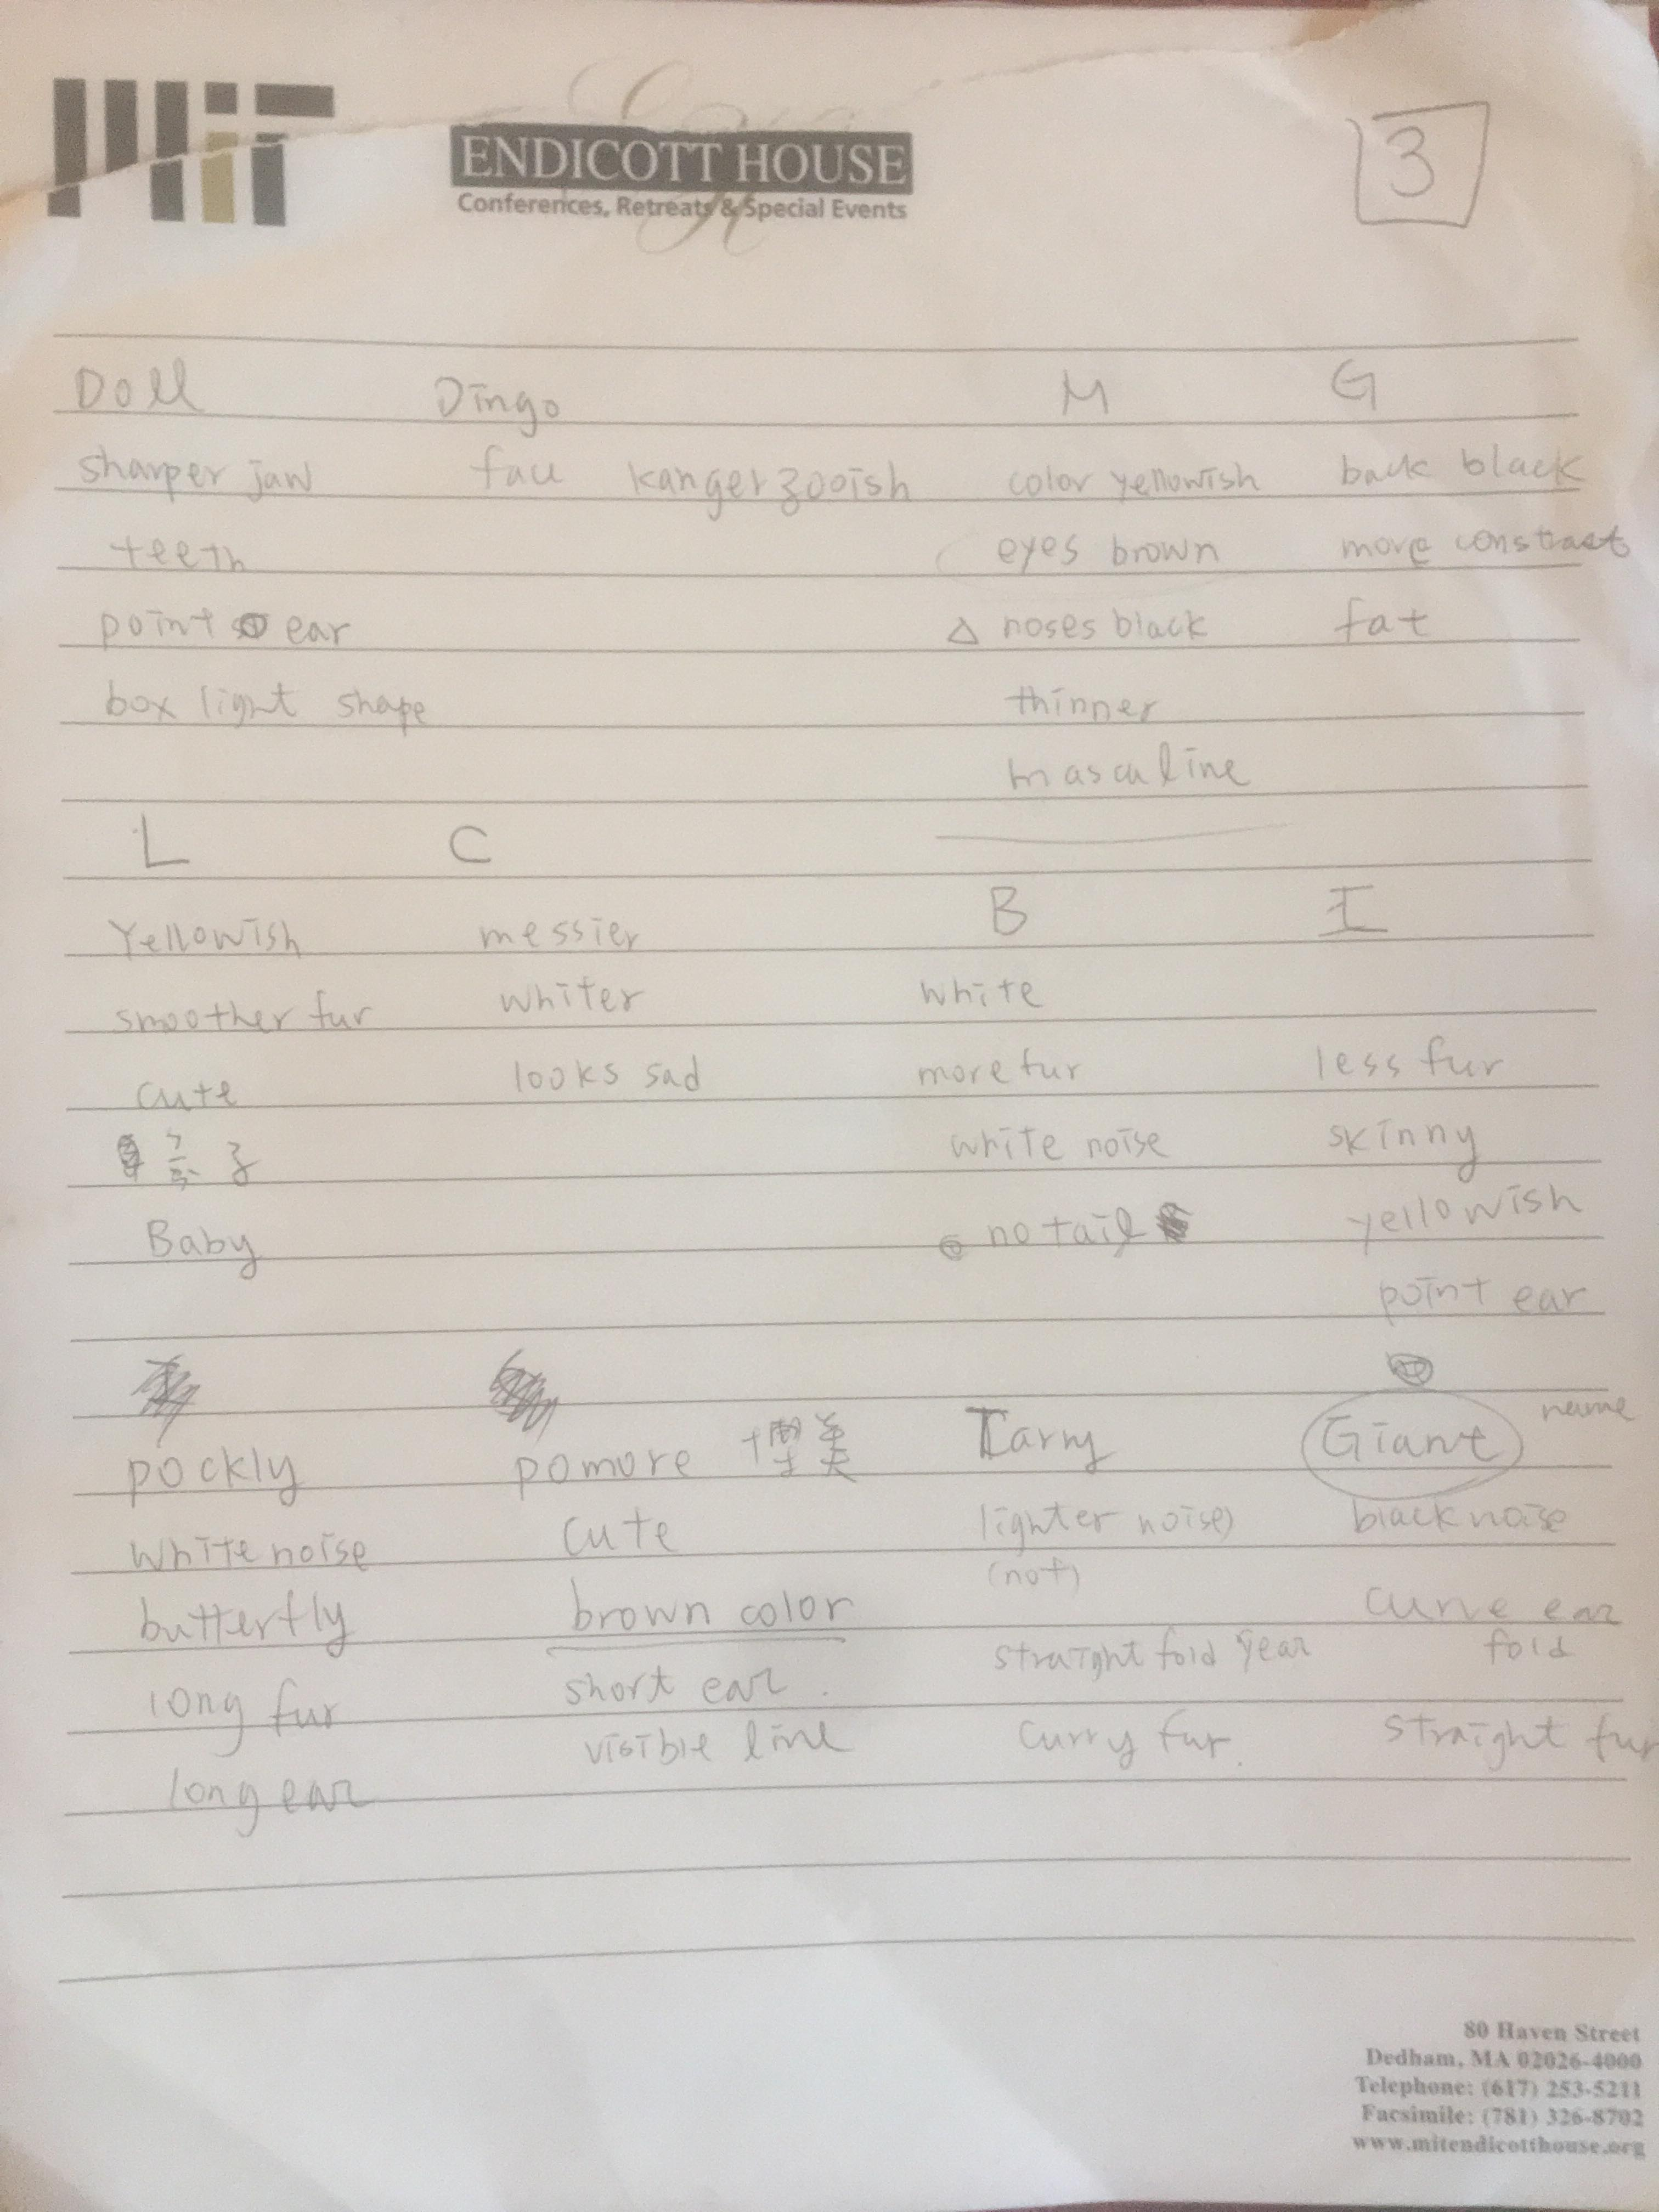
\includegraphics[width=0.89\textwidth]{images/notes-3.jpg}}
    \caption{Notes taken by a member of team 3.}
    \label{fig:notes3}
\end{figure*}

\end{document}
